\chapter{Context-Free Grammars}

\section{Motivation}

Regular languages cannot describe nesting. Balanced parentheses, nested blocks and
arithmetic expressions all require ``memory'' of unbounded depth. Context-free grammars
(CFGs) add recursion, which is exactly enough to describe the syntactic structure of most
programming languages.

\section{Definitions}

\begin{definition}
A \textbf{context-free grammar} is a 4-tuple $G = (N, T, P, S)$:
\begin{itemize}
  \item $N$: a finite set of \textbf{non-terminals};
  \item $T$: a finite set of \textbf{terminals} (the alphabet, disjoint from $N$);
  \item $P$: a finite set of \textbf{productions} $A \to \alpha$ with $A\in N$,
        $\alpha \in (N\cup T)^*$;
  \item $S\in N$: the \textbf{start symbol}.
\end{itemize}
Let $V = N\cup T$ be the vocabulary.
\end{definition}

Conventions: $a,b,c$ are terminals; $A,B,C,S$ non-terminals; $w,x,y,z \in T^*$;
$\alpha,\beta,\gamma \in V^*$. ``Context-free'' means a non-terminal $A$ can be replaced by
$\alpha$ regardless of what surrounds it.

\begin{definition}
$\alpha A \beta \Rightarrow \alpha\gamma\beta$ (\emph{directly derives}) if $A\to\gamma \in P$.
$\Rightarrow^*$ is the reflexive transitive closure. A \textbf{derivation} of $w$ is a
sequence $S \Rightarrow \alpha_1 \Rightarrow \dots \Rightarrow w$. The language of $G$ is
$L(G) = \{ w \in T^* : S \Rightarrow^* w\}$. A language is \textbf{context-free} if some CFG
generates it.
\end{definition}

\begin{example}
$S \to aSb \mid \varepsilon$ generates $\{a^nb^n : n\ge 0\}$ (not regular).
Balanced parentheses: $S \to (S)S \mid \varepsilon$.
Palindromes over $\{a,b\}$: $S \to aSa \mid bSb \mid a \mid b \mid \varepsilon$.
\end{example}

Every regular language is context-free: a DFA transition $\delta(q,a)=r$ becomes the
production $Q \to aR$, and each accepting state $Q$ gets $Q \to \varepsilon$.

\section{Derivations and parse trees}

Consider
\[
  E \to E + E \mid E * E \mid (E) \mid \mathtt{id}.
\]

A \textbf{leftmost derivation} always expands the leftmost non-terminal; a
\textbf{rightmost derivation} the rightmost:
\begin{align*}
\text{leftmost: } & E \Rightarrow E + E \Rightarrow \mathtt{id} + E \Rightarrow
  \mathtt{id} + E * E \Rightarrow \mathtt{id}+\mathtt{id}*E \Rightarrow \mathtt{id}+\mathtt{id}*\mathtt{id} \\
\text{rightmost: } & E \Rightarrow E + E \Rightarrow E + E * E \Rightarrow
  E + E * \mathtt{id} \Rightarrow E+\mathtt{id}*\mathtt{id} \Rightarrow \mathtt{id}+\mathtt{id}*\mathtt{id}
\end{align*}

A \textbf{parse tree} records which production was applied to each non-terminal, forgetting
the order. Root is $S$; each internal node $A$ with children $X_1\dots X_k$ corresponds to a
production $A\to X_1\dots X_k$; leaves read left-to-right give the derived string. Each parse
tree corresponds to exactly one leftmost and exactly one rightmost derivation.

Top-down parsers (Chapter 9) construct leftmost derivations; bottom-up parsers (Chapter 10)
construct rightmost derivations in reverse.

\section{Ambiguity}

\begin{definition}
A grammar is \textbf{ambiguous} if some word has two distinct parse trees (equivalently,
two distinct leftmost derivations).
\end{definition}

The expression grammar above is ambiguous: $\mathtt{id}+\mathtt{id}*\mathtt{id}$ also has
the leftmost derivation $E\Rightarrow E*E \Rightarrow E+E*E \Rightarrow\dots$

\begin{center}
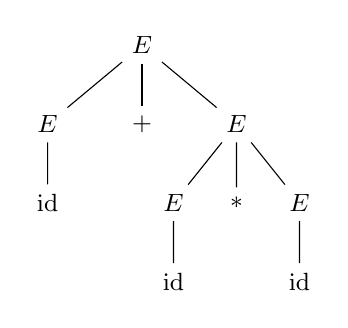
\begin{tikzpicture}[level distance=1cm,
  level 1/.style={sibling distance=1.2cm},
  level 2/.style={sibling distance=0.8cm}, every node/.style={font=\small}]
\node {$E$}
  child {node {$E$} child {node {id}}}
  child {node {$+$}}
  child {node {$E$}
     child {node {$E$} child {node {id}}}
     child {node {$*$}}
     child {node {$E$} child {node {id}}}};
\end{tikzpicture}
\hspace{2cm}
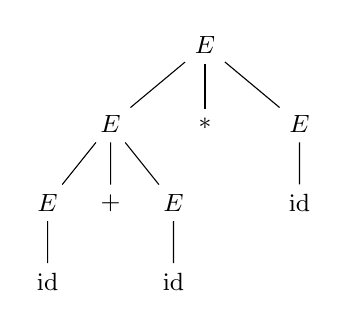
\begin{tikzpicture}[level distance=1cm,
  level 1/.style={sibling distance=1.2cm},
  level 2/.style={sibling distance=0.8cm}, every node/.style={font=\small}]
\node {$E$}
  child {node {$E$}
     child {node {$E$} child {node {id}}}
     child {node {$+$}}
     child {node {$E$} child {node {id}}}}
  child {node {$*$}}
  child {node {$E$} child {node {id}}};
\end{tikzpicture}

\small Left: $a + (b*c)$ (intended). Right: $(a+b)*c$.
\end{center}

Ambiguity matters because a compiler assigns \emph{meaning} by walking the parse tree; two
trees mean two different programs. Note: ambiguity is a property of the \emph{grammar}. Some
context-free languages are \emph{inherently ambiguous} (every grammar for them is ambiguous),
e.g.\ $\{a^ib^jc^k : i=j \text{ or } j=k\}$. Deciding whether a CFG is ambiguous is
undecidable in general.

\section{Precedence and associativity}

Two ways to handle ambiguity: (1) keep the ambiguous grammar and add disambiguation rules to
the parser (as tools like yacc/bison do); (2) rewrite the grammar to be unambiguous. The
standard rewrite introduces one non-terminal per precedence level:
\begin{align*}
  E &\to E + T \mid E - T \mid T \\
  T &\to T * F \mid T / F \mid F \\
  F &\to (E) \mid \mathtt{id}
\end{align*}
\begin{itemize}
  \item \textbf{Precedence}: $*$ is generated lower in the tree (by $T$) than $+$ (by $E$), so it
        binds tighter. Operators lower in the tree are evaluated first.
  \item \textbf{Associativity}: $E\to E+T$ is \emph{left-recursive}, so $a-b-c$ parses as
        $(a-b)-c$ (left-associative). Writing $E\to T + E$ would make it right-associative,
        which is wrong for $-$ and $/$ (but correct for e.g.\ exponentiation or assignment).
\end{itemize}

\begin{example}
Parse tree of $a - b * c$ in the unambiguous grammar:
\begin{center}
\begin{tikzpicture}[level distance=0.9cm,
  level 1/.style={sibling distance=1.6cm},
  level 2/.style={sibling distance=1cm},
  level 3/.style={sibling distance=0.8cm}, every node/.style={font=\small}]
\node {$E$}
  child {node {$E$} child {node {$T$} child {node {$F$} child {node {$a$}}}}}
  child {node {$-$}}
  child {node {$T$}
     child {node {$T$} child {node {$F$} child {node {$b$}}}}
     child {node {$*$}}
     child {node {$F$} child {node {$c$}}}};
\end{tikzpicture}
\end{center}
\end{example}

\paragraph{The dangling else.} $S \to \mathtt{if}\ E\ S \mid \mathtt{if}\ E\ S\ \mathtt{else}\ S
\mid \dots$ is ambiguous for \code{if a if b x else y}. The convention is ``else matches the
nearest unmatched if''. WLP4 sidesteps the issue by requiring braces and always having an else:
\code{if (test) \{ stmts \} else \{ stmts \}}.

\section{The WLP4 grammar (excerpt)}

WLP4 (``Waterloo, Language Plus Pointers Plus Procedures'') is the C-like language we compile.
A fragment of its grammar:
\begin{lstlisting}
start     -> BOF procedures EOF
procedures-> procedure procedures | main
procedure -> INT ID LPAREN params RPAREN LBRACE dcls statements RETURN expr SEMI RBRACE
main      -> INT WAIN LPAREN dcl COMMA dcl RPAREN LBRACE dcls statements RETURN expr SEMI RBRACE
dcl       -> type ID
type      -> INT | INT STAR
dcls      -> | dcls dcl BECOMES NUM SEMI | dcls dcl BECOMES NULL SEMI
statements-> | statements statement
statement -> lvalue BECOMES expr SEMI
           | IF LPAREN test RPAREN LBRACE statements RBRACE ELSE LBRACE statements RBRACE
           | WHILE LPAREN test RPAREN LBRACE statements RBRACE
           | PRINTLN LPAREN expr RPAREN SEMI
           | DELETE LBRACK RBRACK expr SEMI
test      -> expr EQ expr | expr NE expr | expr LT expr | ...
expr      -> term | expr PLUS term | expr MINUS term
term      -> factor | term STAR factor | term SLASH factor | term PCT factor
factor    -> ID | NUM | NULL | LPAREN expr RPAREN | AMP lvalue | STAR factor
           | NEW INT LBRACK expr RBRACK | ID LPAREN RPAREN | ID LPAREN arglist RPAREN
\end{lstlisting}
Note the \code{expr}/\code{term}/\code{factor} layering, exactly the precedence technique above.
\code{BOF} and \code{EOF} are artificial tokens that make parsing algorithms cleaner.

\section{Parsing as a problem}

\textbf{Parsing}: given $G$ and $w$, decide whether $w\in L(G)$ and, if so, produce a
derivation (parse tree). General algorithms (CYK, Earley) run in $\bigO(n^3)$ time, too
slow for compilers. Instead we restrict to grammar classes that allow linear-time parsing
with one token of lookahead: LL(1) (top-down) and LR(1)/LALR(1) (bottom-up).

\section{Summary}
\begin{itemize}
  \item CFG $=(N,T,P,S)$; derivations replace one non-terminal at a time.
  \item Parse trees abstract away derivation order; leftmost and rightmost derivations are
        canonical orders.
  \item Ambiguous grammar: some string has two parse trees, hence two meanings.
  \item Encode precedence with one non-terminal per level; left recursion gives left associativity.
  \item WLP4's grammar uses \code{expr}/\code{term}/\code{factor}; BOF/EOF delimit the input.
\end{itemize}
